%!TEX TS-program = ../make.zsh

\subsection{Hole-Ice Propagation With a Generalized Medium-Propagation Algorithm to Replace the Existing Propagation Algorithm}
\label{sec:algorithm_b}

% https://github.com/fiedl/hole-ice-study/issues/78

A second approach to adding propagation through hole-ice cylinders to the standard propagation algorithm (section \ref{sec:standardphotonpropagationalgorithm}) implemented in \clsim is to rewrite the part of the algorithm that propagates the photon through different media, aiming to make this algorithm more generic and support hole-ice cylinders at the same level as other structures such as ice layers.

\sourcepar{The source code of the implementation of this second approach can be found in appendix \ref{sec:algorithm_b_source} as well as in the code repository at \url{https://github.com/fiedl/clsim/tree/sf/hole-ice-2018/resources/kernels/lib}.}

In order to propagate a photon through different media, the standard propagation algorithm converts the randomized number of interaction lengths $N$ into a geometrical distance $X:=\sum_i n_i\,\lambda_i,\ N = \sum_i n_i$ (equation \ref{eq:convertbudgettodistance} on page \pageref{eq:convertbudgettodistance}) based on the interaction lengths $\lambda_i$ of the different media. In its current implementation in \clsim, however, this conversion is hard-coded in a way that does support medium changes in the form of tilted ice layers but does not support other shapes such as cylinders of hole ice.\footnote{A comparison of the flow charts of standard \clsim's media-propagation algorithm and the new media-propagation algorithm is given in appendix \ref{sec:flow_charts}.}

In the approach described in this section, the medium-propagation algorithm is re-implemented in a way that does support cylinder-shaped media.

\paragraph{Task}
The task of this new \textbf{medium-propagation algorithm} is to determine in each simulation step, which media, including ice layers as well as hole-ice cylinders, are on the photon's path along its current direction and to convert the randomized scattering and absorption length budgets to geometrical distances according to the interaction lengths of the different media.

\paragraph{Context}
The new medium-propagation algorithm is inserted into the \clsim propagation algorithm's simulation step right after \clsim has randomized the number of scattering lengths to the next scattering point, replacing \clsim's original medium-propagation algorithm. After the medium-propagation algorithm follows the check whether the photon hits an optical module on the way from the current scattering point $A$ to the next scattering point $B$.

The medium-propagation algorithm takes the following input parameters: Current photon position at point $A$, photon direction after scattering at point $A$, a list of the hole-ice cylinders with their coordinates, radii, scattering lengths and absorption lengths, a list of ice layers with their coordinates, scattering lengths and absorption lengths, the randomized number of scattering lengths to the next scattering point, the remaining number of absorption lengths to the absorption point, and the remaining geometric distance to absorption.

As output parameters, the medium-propagation algorithm returns the updated number of remaining absorption lengths to the absorption point, the geometric distance to the next scattering point, and the updated remaining geometric distance to absorption.

\paragraph{Procedure}
The new algorithm works with a generic list of media. For each medium, the algorithm stores the scattering length, the absorption length, and the distance along the photon's direction from the current photon position to the medium's border. This way, the algorithm knows in which distance from the current position which medium's properties take effect.

Due to this generic structure, homogeneous media with all kinds of shapes could be added to this list. In this first implementation, the algorithm adds un-tilted ice layers and cylinders, which model hole ice and cables. Tilted ice layers as well as absorption anisotropy are not re-implemented in this first implementation, but may be added later.\footnote{At the time of writing, ice tilt and absorption anisotropy are not re-implemented, yet. To check the current state of this issue, see \url{https://github.com/fiedl/hole-ice-study/issues/48}.}

After adding ice layers and hole-ice cylinders to the media list, the algorithm sorts the list by ascending distance from the current photon position in order to have the list in the proper order for the following calculations.

Finally, the algorithm loops over the media list and calculates the geometrical distances to the next scattering point and to the absorption point just like the previous media-propagation algorithm has done for ice layers only.

% - Beim Übergang von A nach B kann man die Zwischenschritte visualisieren: z.B. ohne Layers etc. 2018-03-09
% - rewrite #45 2018-03-09 2018-03-10
% - clsim und ppc berechnen mit ais und aia in welchem layer das photon interagiert. dann umrechnung in geometrische längen. B macht das in einer loop.

\paragraph{Media Loop}
In the loop over the different media along the photon's direction, the algorithm calculates the contribution of the media to the geometrical distances to the next scattering point and to the absorption point.

The flow chart of the whole media loop is shown in figure \ref{fig:nimuriX4}. The flow chart for the calculation of one medium's contribution is shown separately in figure \ref{fig:eewoo3Be}.

\begin{figure}[p]
  \resizebox{\textwidth}{!}{%
    \begin{tikzpicture}
  [
    %scale=1,
    node distance = 1.8cm,
    every node/.style = {fill=white, font=\sffamily},
    align = center
  ]

  % Nodes
  \newcommand\process[3]{\node(#1)[process, #3]{#2}}
  \newcommand\decision[3]{\node(#1)[decision, #3]{#2}}
  \node(start)[start]{Start};
  \decision{boundaryleft}{Medium\\boundary left\\?}{below = 2cm of start};

  \process{next}{Take next medium boundary}{right = 4cm of boundaryleft};
  \process{scadistance}{Calculate contribution of this medium\\up to the next medium boundary\\to the geometrical distance to the\\next \textbf{scattering} point}{below of = next};
  \process{absdistance}{Calculate contribution of this medium\\up to the next medium boundary\\to the geometrical distance to \textbf{absorption}}{below = 5mm of scadistance};

  \process{spendrestsca}{Calculate contribution of the last medium\\to the geometrical distance to the next scattering point}{below = 5cm of boundaryleft};
  \process{spendrestabs}{Calculate contribution of the last medium\\to the geometrical distance to absorption}{below of = spendrestsca};

  \decision{ifabsorbed}{Distance to\\absorption reached\\?}{below = 5mm of spendrestabs};
  \process{propagateonlytoabs}{Only propagate to the absorption point}{right = 2.5cm of ifabsorbed};

  \node(return)[stop, below = 2cm of ifabsorbed]{Return};

  % % Comments
  \newcommand\comment[2]{\node ()[substeps, right = 1mm of #1]{#2}}
  \comment{start}{
    \substep number of scattering lengths left to next scattering point\\
    \substep number of absorption lengths left to absorption\\
    \substep list of media. Each: distance to medium boundary, local scattering lenght, local absorption length
  };
  \comment{return}{
    \substep geometrical distance to next scattering point\\
    \substep geometrical distance to absorption
  };

  % Curly braces
  \makeatletter
    \@ifundefined{r@fig:eewoo3Be}{}{
      \draw [decorate, decoration={brace,amplitude=10pt,raise=4pt}, yshift=0pt]
        (absdistance.west) -- +(0,2.5) node [midway,xshift=-1.8cm] {See figure \ref{fig:eewoo3Be}};
    }
  \makeatother

  % Arrows
  \newcommand\connect[2]{\draw[->](#1)--(#2)}
  \connect{start}{boundaryleft};
  \connect{boundaryleft}{next};
  \connect{next}{scadistance};
  \connect{scadistance}{absdistance};
  \draw [->] (absdistance) |- +(5,-1.5) |- (0,-1.5);

  \connect{boundaryleft}{spendrestsca};

  \connect{spendrestsca}{spendrestabs};
  \connect{spendrestabs}{ifabsorbed};
  \connect{ifabsorbed}{propagateonlytoabs};
  \draw [->] (propagateonlytoabs) |- (0,-20.0);

  \connect{ifabsorbed}{return};

  % YES/NO labels
  \node () [right = 1mm of boundaryleft, yshift = 3mm] {YES};
  \node () [below = -1mm of boundaryleft, xshift = -5mm] {NO};

  \node () [right = 1mm of ifabsorbed, yshift = 3mm] {YES};
  \node () [below = -1mm of ifabsorbed, xshift = -5mm] {NO};

\end{tikzpicture}

  }
  \vspace*{5mm}
  \caption{Flow chart of the part of the new media-propagation algorithm that loops over list of media and calculates geometrical distances to the next scattering point and to the absorption point.}
  \label{fig:nimuriX4}
\end{figure}

% \todo{In figure \ref{fig:nimuriX4}, it is not clear how the media loop determines the last medium: Does the photon scatter or be absorbed in this medium?}

\begin{figure}[htbp]
  \image{algorithm-media-loop-2018-calculation}
  \caption{Flow chart of the part of the new media-propagation algorithm that calculates the contribution of one specific medium to the geometrical distances to next scattering point and to the absorption point.}
  \label{fig:eewoo3Be}
\end{figure}

\paragraph{Contribution of the Last Medium}
As shown in figure \ref{fig:nimuriX4}, the last medium is handled separately as the contribution of the last medium is not determined by the size of the medium but by the amount of scattering and absorption budget left.

The contributions of the first $(m-1)$ media to the geometrical distance sum up to $\sum_{i=1}^{m-1} x_i$ where each contribution $x_i := n_i\,\lambda_i$ determines how much of the budget $N:=\sum_{i=1}^m n_i$ is spent. After the first $(m-1)$ media have been crossed, $n_m := N - \sum_{i=1}^{m-1} n_i$ of the budget is left for the last medium. Thus, the photon travels a distance of $x_m := n_m\,\lambda_m$ in the last medium where it reaches the interaction point.

\paragraph{Absorption Before Reaching the Scattering Point}
When calculating the distance to the next scattering point based on the scattering length budget, if the photon's absorption length budget is spent before reaching the next scattering point, that is to say if the distance from the current scattering point $A$ to the absorption point is shorter than the distance from $A$ to the next scattering point, then the next trajectory point $B$ is set to be the absorption point as shown in figure \ref{fig:nimuriX4}. The final trajectory point of the photon is its point of absorption.

\paragraph{Scattering Before Reaching the Absorption Point}
When calculating the contribution of a medium to the remaining distance to the absorption point as shown in the lower half of figure \ref{fig:eewoo3Be}, the algorithm needs to know what distance $\gamma$ within that medium contributes to spending the absorption length budget.

If the photon does not scatter within this medium, the distance $\gamma$ is just the distance from one medium border to the next medium border along the photon direction.\footnote{This corresponds to the termination point being set to the second intersection point, $C = X$, in Case 4 and Case 5 of the hole-ice-correction algorithm described in section \ref{sec:algorithm_a}.}
If the photon does scatter within this medium, the distance $\gamma$ is set to the distance to the scattering point\footnote{This corresponds to the termination point being set to the point of the other interaction in Case 4 and Case 5 of the hole-ice-correction algorithm described in section \ref{sec:algorithm_a}.} as shown in the upper half of figure \ref{fig:eewoo3Be}.

\paragraph{Order and Precedence of Cylinders}

\begin{figure}[htbp]
  \subcaptionbox{In a case where the inner cylinder is smaller, intuition suggests that the inner cylinder represents a special area within a more general area and should take precedence for a photon located within both cylinders.}{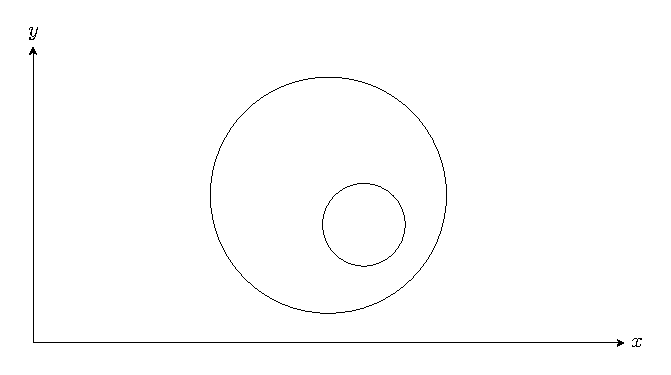
\includegraphics[width=0.48\textwidth]{img/cylinder-order-kuZ8deek}}\hfill
  \subcaptionbox{If both overlapping cylinders have the same size, the choice which properties should be applied to a photon at a position within the overlap of both cylinders, is arbitrary. }{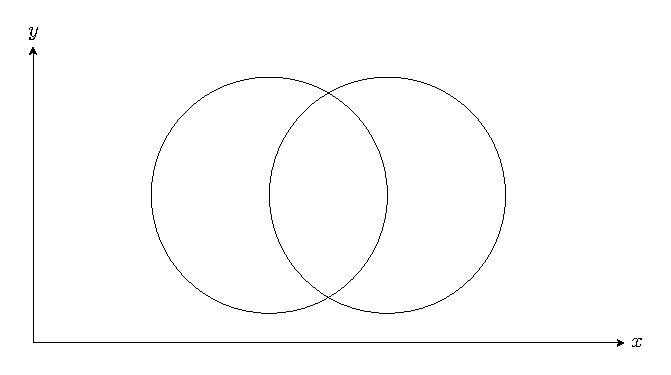
\includegraphics[width=0.48\textwidth]{img/cylinder-order-Yeifohm3}}
  \caption{Two-dimensional projection of nested or overlapping hole-ice cylinders with different ice properties. If a photon is at a position within the overlap of both cylinders, which ice properties should be applied for the propagation? The algorithm defines that the cylinder added last takes precedence.}
  \label{fig:kuZ8deek}
\end{figure}

When nesting or overlapping cylinders as shown in figure \ref{fig:kuZ8deek}, the algorithm needs to determine which ice properties to apply for a photon at a position within both cylinders.

In the left part (a) of the figure, the intuition might be: The smaller cylinder models a special area within the more general outer cylinder and, therefore, should take precedence. In the right part (b) of the figure, however, both cylinders have the same size. Here it is unclear which ice properties to apply for a position within the cylinders' overlap.

To make this situation unambiguous, the algorithm defines that the media added to the list later take precedence over media added earlier. Therefore, when modeling nested cylinders, the algorithm requires to add the larger cylinder before adding the smaller cylinder to the definition list.

\paragraph{Pros and Cons}
This second approach allows to define cylinder-shaped areas with absolute scattering and absorption lengths, which meets the requirements of the current understanding of the hole-ice phenomenon.

Simulation steps over large $z$-distances that cross hole-ice cylinders are handled well by this algorithm in contrast to the previously described hole-ice-correction algorithm (section \ref{sec:algorithm_a}).

Additionally, this algorithm supports nested or overlapping cylinders, which can be utilized to model bubble column together with the drill-hole column as well as the string's cable.

Ice tilt and absorption anisotropy have not been ported to this algorithm, yet, but can be added later on.\footnote{See: \url{https://github.com/fiedl/hole-ice-study/issues/48}.}

The down side to this approach is that an important part of standard-\clsim's media-propagation algorithm needed to be re-implemented, requiring evidence that the new algorithm is still doing what is expected. In order to provide this evidence, section \ref{sec:unit_tests_and_cross_checks} describes a series of cross checks to make sure the new algorithm results in the expected scattering and absorption behavior.

Also, standard-\clsim's medium-propagation has been ported to the new interfaces as drop-in replacement for the new medium-propagation algorithm, such that one can switch between both algorithms without a code rollback.\footnote{A guide on how to switch the medium-propagation algorithm is presented in appendix \ref{sec:how_to_switch_media_propagation}.}

\begin{table}
  \begin{tabelle}{l|L|L}
    & \textbf{Algorithm (a)} & \textbf{Algorithm (b)} \\
    \hline
    Approach
      & Leave \clsim medium propagation as it is and add \textbf{hole-ice effects as correction} afterwards
      & Unify \clsim medium propagation through layers and hole ice: Treat them as \textbf{generic medium changes} \\
    Hole-ice properties
      & defined relative to bulk-ice properties
      & defined absolute \\
    Pros
      &
        \begin{itemize}
          \item[+] Small surface area of hole-ice code, well testable through unit tests
          \item[+] Standard \clsim almost untouched
        \end{itemize}
      &
        \begin{itemize}
          \item[+] Supports nested cylinders and cables
        \end{itemize}
      \\
    Cons
      &
        \begin{itemize}
          \item[--] Current understanding of hole-ice suggests defining hole-ice properties absolute rather than relative
        \end{itemize}
      &
        \begin{itemize}
          \item[--] Needed rewrite of \clsim's medium-propagation code
          \item[--] Ice tilt and ice anisotropy not re-implemented, yet
        \end{itemize}
  \end{tabelle}
  \caption{Comparison of the hole-ice-correction algorithm (a) presented in section \ref{sec:algorithm_a} and the new generic medium-propagation algorithm (b) presented in section \ref{sec:algorithm_b}.}
\end{table}

A comparison to other methods to account for the hole-ice effect is presented in section \ref{sec:comparison_methods}.